\chapter{結果}\chaplab{result}
本章では,\chapref{methods}で述べた推定の結果を,重み付き平均,MAP推定に分けて述べる.
\section{重み付き平均}
ランダムに分割したテストデータ32個に対し,各時刻に推定を行い,各時刻の重み付き平均を推定時刻として出力した.tabrefである.
\begin{table}[htb]
  \begin{center}
    \begin{tabular}{|l||c|r|} \hline
       & 第一主成分 & 第二主成分 \\ \hline
      寄与率 & 0.979 & 0.013 \\ \hline
    \end{tabular}
  \end{center}
\end{table}

概ね
であろう.
また,推定を開始した段階において,5秒前付近であるとする推定結果が多く見られるが,これは,推定結果を重み付き平均として出す関係上,推定の結果が分布の中心点に引っ張られてしまいやすいという特性が存在しているためである.
\par
次に,同様に分割したテストデータに対して推定を行い,MAP推定により推定時刻を出力した.tabrefである.
\begin{table}[htb]
  \begin{center}
    \begin{tabular}{|l||c|r|} \hline
       & 第一主成分 & 第二主成分 \\ \hline
      寄与率 & 0.979 & 0.013 \\ \hline
    \end{tabular}
  \end{center}
\end{table}

MAP推定による結果は,概ね以下の傾向に分かれていることがわかる.
\begin{itemize}
	\item 最初から最後まで正確に推定を続けているもの
	\item 最初から最後まで直前であると推定し続けているもの
	\item 途中から推定結果が改善されるもの
\end{itemize}
まず,正確に推定を続けているものや,途中から推定結果が改善されるものについては,本研究手法の有用性を示すものであると考えられる.しかし,推定を続けていっても常に直前であるという推定結果が混ざってしまうという問題点も抱えており,
MAP推定の問題点はここにある.





MAPでは,最初ほど結果が良い
重み付きでは,車線変更開始直前のほうが良い
MAPでは,一部車線変更直前であると張り付いてしまった.
おもみつきでは...
\par
% 最後に,32個のテストデータに対する更新を30回繰り返したものから,MAPと重み付き平均両方の推定結果を比較した図が,\figref{result}である.
% \begin{figure}[htbp]
  \centering
    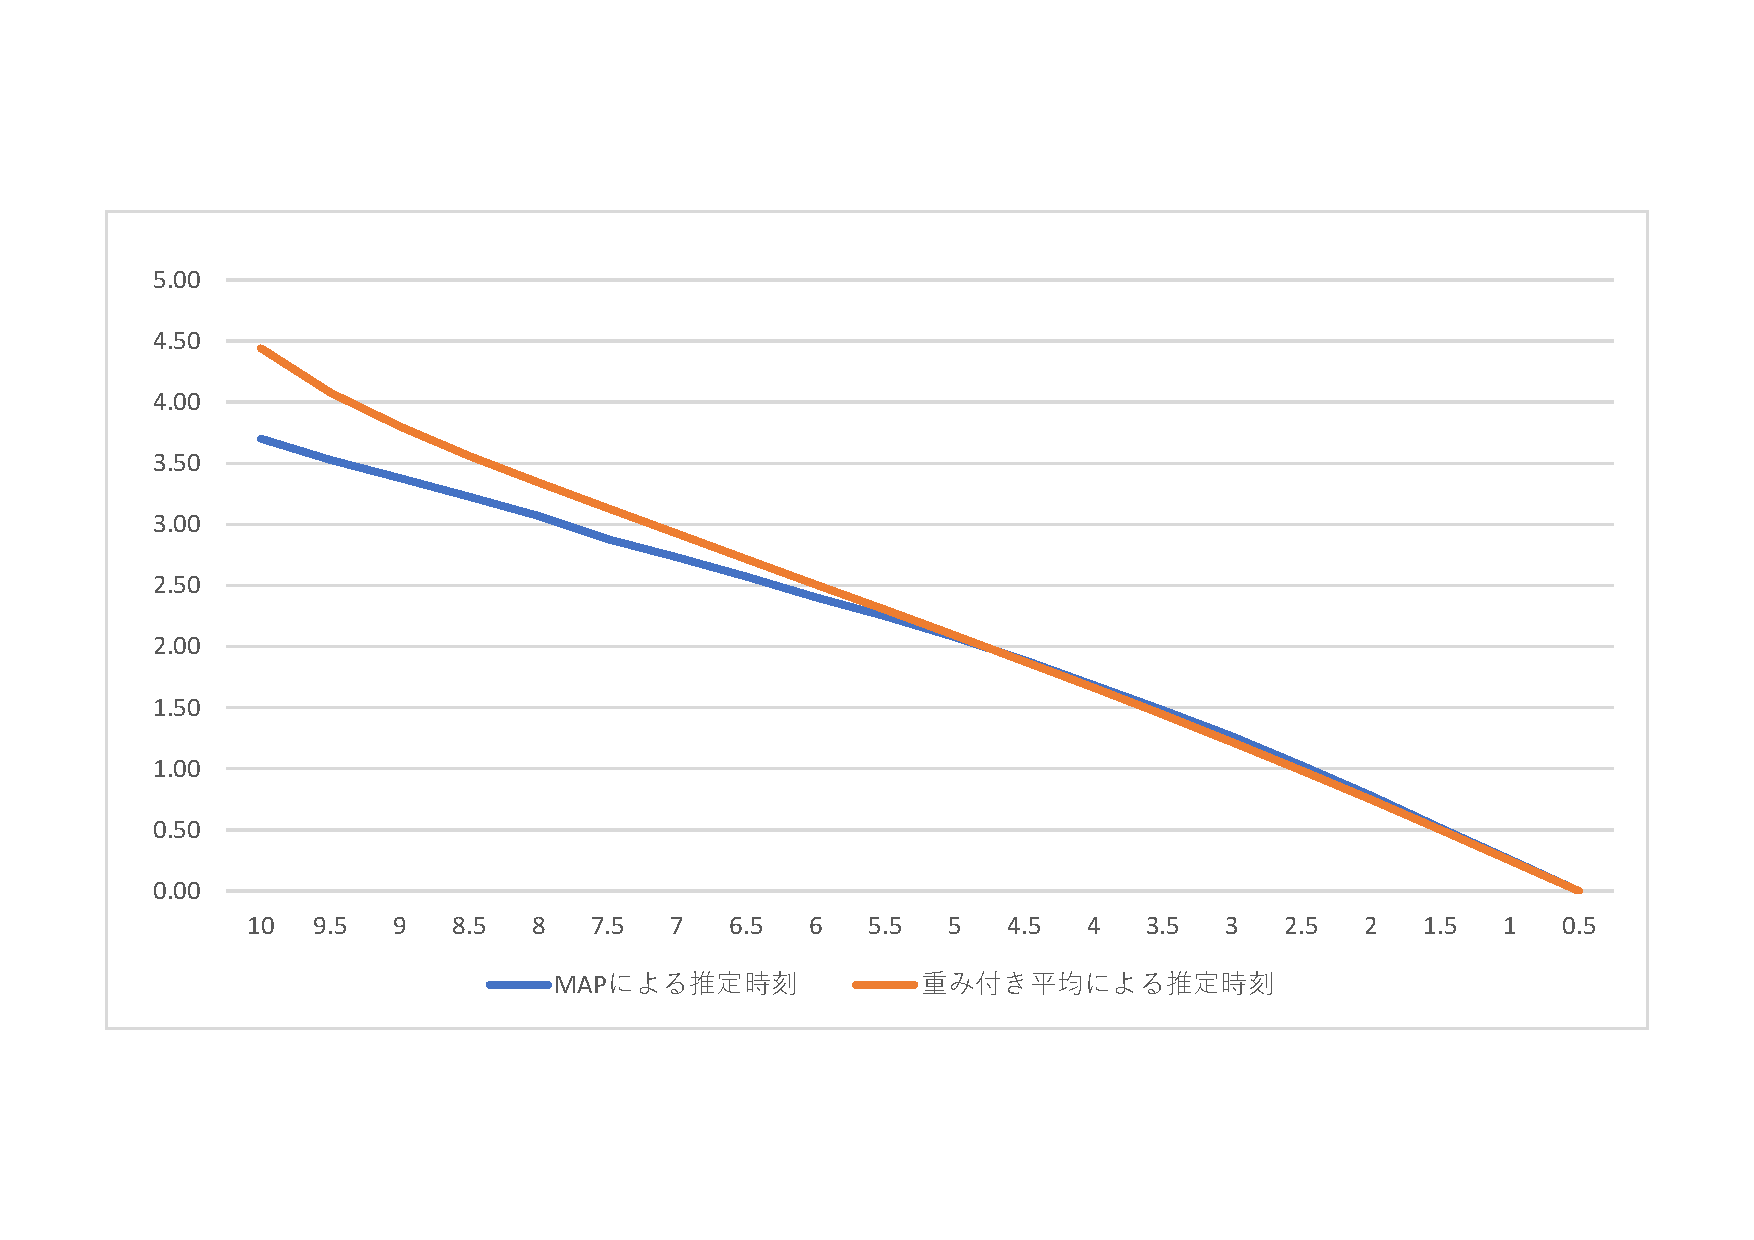
\includegraphics[width=70mm]{fig/result.pdf}
  \caption{result}
  \label{fig:result}
\end{figure}

オレンジの線がMAP推定の誤差を,青の線が重み付き平均による推定の誤差を表している.x軸は実際の車線変更開始までの時間を表している.図から,車線変更の開始が近づき観測点が増えていくにつれて徐々に推定結果が改善されていっていることが読み取れる.
また,車線変更開始5秒まではMAP推定のほうが平均的に良い結果となり,それ以降は重み付き平均のほうが若干ながら良い結果になった.これは,重み付き平均の中心点に引き寄せられやすいという特性に起因している.
